\ref{eq: Lk2}'\section{Realizability problems for RPDA and RPDT}
% Let $\Com_v=\{\pop,\skip,\push\}$ and $v:\Com([k])\to\Com_v$ be the function such that $v(\push(j))=\push$ for $j\in[k]$ and $v(\com)=\com$ otherwise.
% We say that an $(m,k)$-RPDA $\calA$ visibly manipulates its stack (or a {\em visibly} RPDA) if its input and output alphabets are
% $\Sigma_\dblI\times\Com_v$ and $\Sigma_\dblO\times\Com_v$, respectively,
% and every rule of $\calA$ has the form $(q,(a,v(\com)),\tst)\to(q',\asgn,\com)$.
% Let \DRPDAv\ be the union of visibly $k$-DRPDA for all $k\in\Natz$, respectively.


\subsection{Finite actions}
In \cite{EFR19}, the abstraction of the behavior of $k$-register transducer ($k$-RT), called finite actions, was introduced
to reduce the realizability problem for register automata (RA) and RT to
the problem on finite alphabets.
We extend the idea of \cite{EFR19} and define the finite actions of $k$-RPDT.

For $k\in\Natz$,
we define the set of finite input actions as $A_k^\dblI = \Sigma_\dblI\times \Tst_k$
and the set of finite output actions as $A_k^\dblO = \Sigma_\dblO\times \Asgn_k\times [k]\times \Com([k])$.
Note that $\Com([k])$ appearing in the definition of $A_k^\dblO$ is not the abbreviation of $\Com(\Gamma\times[k])$.
Finite actions have no information on finite stack alphabet $\Gamma$ even if $\Gamma$ is not a singleton.
A sequence $w = (a^\dblI_0,d^\dblI_0) (a^\dblO_0,d^\dblO_0)\cdots \in \DW(\Sigma_\dblI,\Sigma_\dblO,D)$ is \emph{compatible} with a sequence
$\overa = (a^\dblI_0, \tst_0)(a^\dblO_0,\asgn_0,j_0, \com_0)\cdots \in (A_k^\dblI\cdot A_k^\dblO)^\omega$
iff there exists a sequence $(\theta_0,u_0)(\theta_1, u_1)\cdots\in (\Theta_k\times D^*)^\omega$, called a \emph{witness}, such that
$\theta_0 = \theta^{k}_\bot$, $u_0 = \bot$,
$(\theta_i, d^\dblI_i, u_i(0)) \models \tst_i, \theta_{i+1}=\theta_i[\asgn_i\leftarrow d^\dblI_i], \theta_{i+1}(j_i) = d^\dblO_i$ and $u_{i+1}=\upds(u_i,\theta_{i+1},\com_i)$.
Let $\Comp(\overa) = \{w\in \DW(\Sigma_\dblI,\Sigma_\dblO,D)\mid$ $w$ is compatible with $\overa$ $\}$.
For a specification $S \subseteq \DW(\Sigma_\dblI,\Sigma_\dblO,D)$, we define $W_{S,k}=\{\overa\mid \Comp(\overa)\subseteq S\}$.

For a data word
$w\in\DW(\Sigma_\dblI,\Sigma_\dblO,D)$ and
a sequence $\overa\in(A_k^\dblI\cdot A_k^\dblO)^\omega$
such that
for each $i\geq 0$, there exists
$a\in\Sigma$
and we can write
$w(i)=(a,d)$ and $\overa(i)=(a,\tst)$ if $i$ is even
and $\overa(i)=(a,\asgn,j,\com)$ if $i$ is odd,
we define $w\otimes\overa\in\DW(A_k^\dblI,A_k^\dblO,D)$ as
$w\otimes\overa(i)=(\overa(i), d)$ where $w(i)=(a,d)$.
% We call an $(m,k)$-DRPDA $\calA$ over $A^\dblI_k,A^\dblO_k$ and $\Gamma$
% visible if
% Finite actions $A^\dblI_k$ and $A^\dblO_k$
% uniquely determine an alphabet
% $A^\dblI'=\{\}\subseteq(\Sigma_\dblI\times \Tst_k)$ and
% $A^\dblO_k$
% We assume $(m,k)$-DRPDA $\calA$ over $A^\dblI_k,A^\dblO_k$ and $\Gamma$
% is visible, or $\calA$ is visibly $(m,k)$-DRPDA,
% if every rule of $\calA$ has one of the forms
% $(q, (a, \skip, \tst'), \tst) \to (q', \asgn, \skip)$ and
% $(q, (b, v(\com), \asgn', j, \com'), \tst) \to (q', \asgn, \com)$.
% Note that $\calA\in\DRPDAv$\ always holds.

\subsection{Decidability and undecidability of realizability problems}
\begin{lemma}\label{lem: Lk}
$L_k = \{w\otimes\overa \mid w\in\Comp(\overa)\}$ is definable as the language of a $(2,k+2)$-DRPDA.
\end{lemma}
{\bf Proof sketch.}\quad
Let $(2,k+2)$-DRPDA
$\calA_1=(Q_1, Q^\dblI_1, Q^\dblO_1, p, \delta_1, c_1)$
over $A_k^\dblI, A_k^\dblO$ and $\Gamma$ where
$Q_1=\{p, q\}\cup(\Asgn_k\times[k]\times\Com([k]))\cup[k]$, $Q^\dblI_1=\{p\}$, $Q^\dblO_1 = Q_1\setminus Q^\dblI_1$,
$c_1(s)=2$ for every $s\in Q$ and $\delta_1$ consists of all the rules of the form
\begin{align}
(p, (a_\dblI, \tst), \tst\cup\tst')&\to(q, \{k+1\}, \skip)\label{eq: Lk1}\\
(q, (a_\dblO, \asgn, j, \com), \tst'')&\to((\asgn,j,\com), \{k+2\},\skip)\label{eq: Lk2}\\
((\asgn,j,\com), \tau, \{k+1\}\cup\tst'')&\to(j, \asgn, \com)\label{eq: Lk3}\\
(j, \tau, \{j, k+2\}\cup\tst'')&\to(p, \emptyset, \skip)\label{eq: Lk4}
\end{align}
for $(a_\dblI, \tst)\in A_k^\dblI$, $(a_\dblO, \asgn, j, \com)\in A_k^\dblO$, $\tst'\subseteq \{k+1,k+2\}$ and $\tst''\in\Tst_{k+2}$.
As in Fig. \ref{fig: lem_Lk},
$\calA_1$ checks whether an input sequence satisfies the conditions of compatibility
by nondeterministically generating a candidate of a witness of the compatibility step by step.
% We can show $L(\calA_k)=L_k$
% by checking the simulation in Fig. \ref{fig: lem_Lk}
% is correct.
\begin{figure}[t]
  \centering
  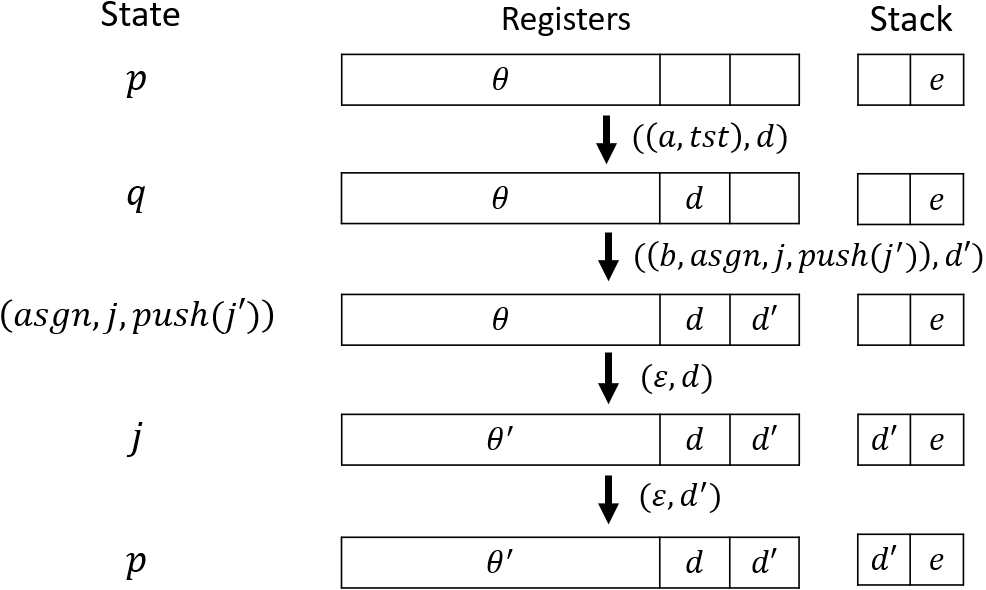
\includegraphics[width=10cm]{lem_Lk.png}
  \caption{An example of transitions of $\calA_k$.}
  \label{fig: lem_Lk}
\end{figure}

\begin{lemma}\label{lem: LkS}
For a specification $\calS$ defined by some visibly $k'$-DRPDA,
$L_{\overS, k} = \{w\otimes\overa \mid w\in\Comp(\overa)\cap \overS\}$
is definable as the language of a $(4,k+k'+4)$-DRPDA.
\end{lemma}
{\bf Proof sketch.}\quad
Let $L_{\overS} = \{w\otimes\overa\mid w\in\overS, \overa\in(A_k^\dblI\cdot A_k^\dblO)^\omega\}$.
Because the class of languages defined by visibly DRPDA is closed under the complement,
we can construct a visibly $k'$-DRPDA
$\calA_2=(Q_2, Q^\dblI_2, Q^\dblO_2, q^0_2, \delta_2, c_2)$
over $A^\dblI_{k}, A^\dblO_{k}$ and $\Gamma$
such that $L(\calA_2)= L_{\overS}$.
Let $\calA_1$ be the $(2,k+2)$-DRPDA
such that $L(\calA_1)=L_k$, which is given in Lemma \ref{lem: Lk}.
Because $L_{\overS, k} = L_{\overS} \cap L_k$, we will construct a $(4,k+k'+4)$-DRPDA $\calA$
over $A^\dblI_{k}, A^\dblO_{k}$ and $\Gamma$
such that $L(\calA)=L(\calA_1)\cap L(\calA_2)$.
We use the properties of $\calA_1$ that
$c_1(q)$ is even for every $q\in Q_1$ and
$\delta_1$ consists of several groups of three consecutive rules having the following forms:
\begin{align}
(q_1, a, \tst_1) &\to (q_2,\asgn_1, \skip) \tag{\ref{eq: Lk2}'}\\
(q_2, \tau, \tst_2) &\to (q_3,\asgn_2, \com_1) \tag{\ref{eq: Lk3}'}\\
(q_3, \tau, \tst_3) &\to (q_4,\asgn_3, \skip) \tag{\ref{eq: Lk4}'}.
\end{align}
Note that $\vis(a)=v(\com_1)$ always holds for such three consecutive rules.
$(\ref{eq: Lk2}'), (\ref{eq: Lk3}')$ and $(\ref{eq: Lk4}')$ correspond to $(\ref{eq: Lk2}), (\ref{eq: Lk3})$ and $(\ref{eq: Lk4})$, respectively, and $(\ref{eq: Lk1})$
is also converted to three consecutive rules like $(\ref{eq: Lk2}')$-$(\ref{eq: Lk4}')$
by adding dummy $\tau$ rules.

We let $k_1=k+2$ and $k_2=k'$.
We construct $(4,k_1+k_2+2)$-DRPDA
$\calA=(Q_\dblI\cup Q_\dblO\cup\{q_0\}, Q_\dblI\cup\{q_0\}, Q_\dblO, q_0, \delta, c)$
where $Q_\dblI=Q^\dblI_1\times Q^\dblI_2\times[5]$,
$Q_\dblO=Q^\dblO_1\times Q^\dblO_2\times[5]$.
$c$ is defined as $c(q_0)=1$ and
$c((q_1,q_2,i))=c_2(q_2)$ for all $(q_1,q_2,i)\in Q$.
$\delta$ has a $\tau$ rule $(q_0,\tau,[k]\cup\{\top\})\to((p, q^2_0,1), \push(1))$.
For all rules (\ref{eq: Lk2}'), (\ref{eq: Lk3}'), (\ref{eq: Lk4}') in $\delta_1$ and
$(q, a, \tst) \to (q',\asgn, \com)\in\delta_2$ (\ref{eq: LkS1})
such that $v(\com_1)=v(\com)\ (=\vis(a))$ for $a\in A^\dblI_{k}\cup A^\dblO_{k}$,
we construct the rules in $\delta$ that
can do the transitions as in Fig. \ref{fig: lem_LkS}.
The figure illustrates an example of transitions of $\calA$
from $(q_1,q,1)$ to $(q_4,q',1)$ with updating
contents of its registers and stack.
The first to $k_1$-th registers simulate
the registers of $\calA_1$,
$(k_1+1)$-th to $(k_1+k_2)$-th registers simulate
the registers of $\calA_2$ and
$(k_1+k_2+1)$-th and $(k_1+k_2+2)$-th registers
are for keeping the first and second stack top contents, respectively.
The stack contents of $\calA$ simulates those of $\calA_1$ and $\calA_2$ by restoring the contents of stacks of $\calA_1$ and $\calA_2$ alternately.
The transition rules from $(q_1,q,1)$ to $(q_1,q,3)$
are for moving the two data values at the stack top
to $(k_1+k_2+1)$-th and $(k_1+k_2+2)$-th registers.
The transition rule from $(q_1,q,3)$ to $(q_2,q',4)$
is for updating states, registers and stacks
by simulating the rules (\ref{eq: Lk2}') and (\ref{eq: LkS1}).
The transition rules from $(q_2,q',4)$ to $(q_4,q',1)$
simulate the rules (\ref{eq: Lk3}') and (\ref{eq: Lk4}'), respectively.
We can show $L(\calA)=L(\calA_1)\cap L(\calA_2)$
by checking the simulation in Fig. \ref{fig: lem_LkS}
is correct.

\begin{figure}[t]
  \centering
  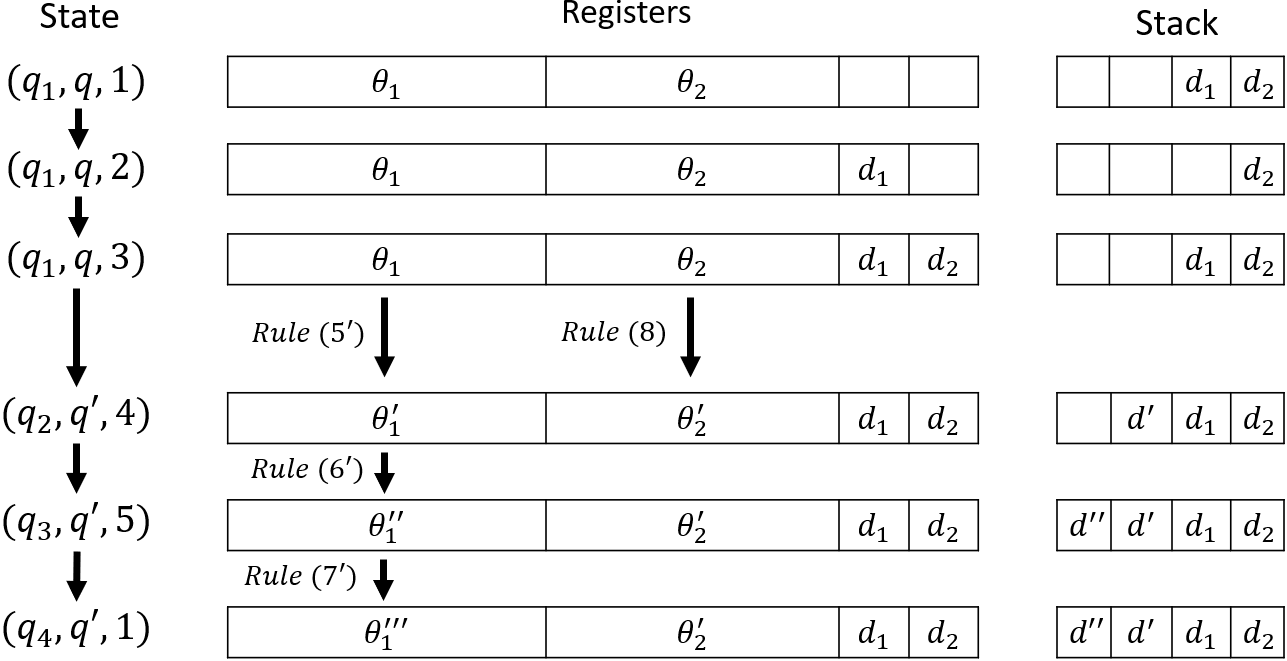
\includegraphics[width=12cm]{lem_LkS.png}
  \caption{An example of transitions of $\calA$ with $\vis(a)=\push$.}
  \label{fig: lem_LkS}
\end{figure}

\begin{lemma} \label{lem: W=lab}
$W_{S,k} = \overline{\lab(L_{\overS,k})}$.
\end{lemma}
{\bf Proof.}\quad
For every $\overa\in(A_k^\dblI A_k^\dblO)^\omega$,
$\overa\notin W_{S,k} \Leftrightarrow \Comp(\overa)\not\subseteq S
\Leftrightarrow \exists w. w\in \Comp(\overa)\cap \overS
\Leftrightarrow \exists w. w\otimes\overa\in L_{\overS,k}
\Leftrightarrow \overa\in\lab(L_{\overS,k})$.
Thus, $W_{S,k} = \overline{\lab(L_{\overS,k})}$ holds.

\begin{theorem}
\label{th: DPDAv}
For all $k\geq 0$, \Real $($\DRPDAv, \RPDTk$)$ is in 2EXPTIME.
\end{theorem}
{\bf Proof.}\quad
By Lemma \ref{lem: LkS} and Theorem \ref{the: RPDAtoPDA},
$W_{S,k}$ is definable by a $4$-DPDA $\calA_f$.
By Lemma \ref{lem: ef}, we can construct a $0$-DPDA $\calA'_f$
where $L(\calA_f')=L(\calA_f)$.
By the construction of $\calA$ in Lemma \ref{lem: LkS},
the stack height of the current ID increases by two during the transitions
from $(q_1,q,1)$ to $(q_4,q',1)$ in Fig. \ref{fig: lem_LkS} if $\vis(a)=\push$,
does not change if $\vis(a)=\skip$ and
decreases by two if $\vis(a)=\pop$.
Thus, $\calA'_f$ is a stack-visibly DPDA,
that is, every transition rule $(p,a,z)\to(q,\com)$ of $\calA'_f$
satisfies $\vis(a)=v(\com)$.
We show the following two conditions are equivalent.
\begin{itemize}
\item There exists a $k$-RPDT $\calT$ such that $L(\calT)\subseteq S$.
\item There exists a PDT $\calT'$ such that $L(\calT')\subseteq W_{S,k}$.
\end{itemize}
Assume that a $k$-RPDT $\calT$ over $\Sigma_\dblI,\Sigma_\dblO$ and $\Gamma$ satisfies $L(\calT)\subseteq S$.
Then, consider the PDT $\calT'$ over $A_k^\dblI,A_k^\dblO$ and $\Gamma$ such that
$(q,(a,\tst),z)\to(q',(b,\asgn,j,\com),\com')$ is a rule of $\calT'$
iff $(q,a,\tst,z)\to(q',b,\asgn,j,\com)$ is a rule of $\calT$ where $\com'=\com$ if $v(\com)=\pop$ or $\skip$ and $\com'=\push(z')$ if $\com=\push(z',j')$ for some $j'\in[k]$.
For $\overa\in L(\calT')$, every $w\in\Comp(\overa)$
has a witness (see Section 6.1) and thus $w\in L(\calT)$ holds.
By the assumption $L(\calT)\subseteq S$,
$\Comp(\overa)\subseteq S$ holds and thus $\overa\in W_{S,k}$.
Hence, we obtain $L(\calT')\subseteq W_{S,k}$.

Conversely, assume there exists a PDT $\calT'$ over $A_k^\dblI,A_k^\dblO$ and $\Gamma$ that
satisfies $L(\calT')\subseteq W_{S,k}$.
We can in particular construct a PDT $\calT''$ such that
$L(\calT'')\subseteq W_{S,k}$ and
every rule $(q,(a,\tst),z)\to(q',(b,\asgn,j,\com),\com')$
satisfies $\vis(b)=v(\com')$
(note that $\vis(a)=\skip$ always holds)
by the construction algorithm in \cite{Wa96}.
In the rule, $v(\com)=v(\com')$ holds because $\calA'_f$ is a stack-visibly PDA and thus $\vis(b)=v(\com)$ holds.
Consider the $k$-RPDT $\calT$ over $\Sigma_\dblI,\Sigma_\dblO$ and $\Gamma$
such that
$(q,a,\tst,z)\to(q',b,\asgn,j,\com'')$ is a rule of $\calT$
iff $(q,(a,\tst),z)\to(q',(b,\asgn,j,\com),\com')$ is a rule of $\calT''$
where $\com''=\com'$ if $\com'=\pop$ or $\skip$ and
$\com''=\push(z',j')$ if $\com'=\push(z')$ and $\com=\push(j')$.
Further, assume $w\in L(\calT)$, and let
$\overa\in (A_k^\dblI\cdot A_k^\dblO)^\omega$
be the sequence with which $w$ is compatible.
Then, by the definition of $\calT$,
$\overa\in L(\calT'')$.
By the assumption $L(\calT'')\subseteq W_{S,k}$,
every $\overa\in L(\calT'')$
satisfies $\Comp(\overa)\subseteq S$, and thus $w\in S$ holds.
Hence, we obtain $L(\calT)\subseteq S$.

By the equivalence, we can check \Real $($\DPDA, \PDT$)$ for $\calA'_f$,
which is shown to be EXPTIME in Theorem \ref{the: DPDA}, instead of checking \Real $($\DRPDAv, \RPDTk$)$.
Because the size of $\calA'_f$ is exponential to $k+k'$,
\Real $($\DRPDAv, \RPDTk$)$ is in 2EXPTIME.
% By Theorem \ref{the: finite_actions}, we can check \Real $($\UPDA, \PDT$)$ for $W_{S,k}$ instead of checking \Real $($\URPDA, \RPDTk$)$.

\begin{theorem}
For all $k\geq 0$, \Real $($\NRPDA, \RPDTk$)$ is undecidable.
\end{theorem}
{\bf Proof.}\quad
We can easily reduce the \Real $($\NPDA, \PDT$)$,
whose undecidability is proved in Theorem \ref{th: NPDA-PDT}, to this problem.


% \section{Realizability problems for Register Automata}
% \subsection{Finite actions}
% For $k\in\Natz$,
% we define the set of finite input actions $A_k^\dblI = \Sigma_\dblI\times \Tst_k$
% and finite output actions $A_k^\dblO = \Sigma_\dblO\times \Asgn_k\times [k]\times \Com([k])$ for $k$-RPDT.
% A sequence $w = (a^\dblI_1,d^\dblI_1) (a^\dblO_1,d^\dblO_1) \cdots \in \DW(\Sigma_\dblI,\Sigma_\dblO,D)$ is compatible with a sequence
% $\overa = (a^\dblI_1,\tst_1)(a^\dblO_1,\asgn_1,j_1, \com_1)\cdots \in (A_k^\dblI A_k^\dblO)^\omega$
% if there exists a run $(\rho, w)$ of $k$-RPDT satisfying follows:
% For all $i\geq 1$, let $\rho(i-1)=(q,\theta,eu)$ and $\rho(i)=(q',\theta',u'u)$
% for some $e\in D, u\in D^*$ and $u'\in D^*$.
% Then $\theta, d^\dblI_i, e\models \tst_i, \theta'=\theta[\asgn_i\leftarrow d^\dblI_i], \theta'(j_1) = d^\dblO_i$ and $u'=Z_D(\com,\theta',e)$ hold.
% Let $\Comp(\overa) = \{w\in \DW(\Sigma_\dblI,\Sigma_\dblO,D)\mid$ $w$ is compatible with $\overa$ $\}$.
% For specification $S \subseteq \DW(\Sigma_\dblI,\Sigma_\dblO,D)$, we define $W_{S,k}=\{\overa\mid \Comp(\overa)\subseteq S\}$.
%
% \begin{theorem}\label{the: finite_actions}
% For a specification $S\subseteq \DW(\Sigma_\dblI,\Sigma_\dblO,D)$, the following statements are equivalent.
% \begin{itemize}
% \item There exists a $k$-RPDT $\calT$ such that $L(\calT)\subseteq S$.
% \item There exists a PDT $\calT'$ such that $L(\calT')\subseteq W_{S,k}$.
% \end{itemize}
% \end{theorem}
%
% % As $A_k^\dblI$ and $A_k^\dblO$,
% % we define the set of finite input actions
% % $\dblA_k^\dblI = \Sigma_\dblI\times \Tst_k\times\Asgn_k\times \Com([k])$
% % and finite output actions
% % $\dblA_k^\dblO = \Sigma_\dblO\times \Tst_k\times\Asgn_k\times \Com([k])$ for $k$-RPDA.
% % A sequence $w = (a^\dblI_1,d^\dblI_1) (a^\dblO_1,d^\dblO_1) \cdots \in \DW(\Sigma_\dblI,\Sigma_\dblO,D)$ is compatible with a sequence
% % $\overa = (a^\dblI_1,\tst_1,\asgn_1,\com_1)(a^\dblO_1,\tst'_1,\asgn'_1,\com'_1)\cdots \in (\dblA_k^\dblI \dblA_k^\dblO)^\omega$
% % if there exists a run $(\rho, w)$ of $k$-RPDA along with conditions appearing in $\overa$.
% % Let $\Comp'(\overa) = \{w\in \DW(\Sigma_\dblI,\Sigma_\dblO,D)\mid$ $w$ is compatible with $\overa$ $\}$.
%
% \subsection{Decidability and undecidability of realizability problems}
% \begin{lemma}
% $L_k = \{w\otimes\overa \mid w\in\Comp(\overa)\}$ is definable as a language of
% $\varepsilon$-equipped $(k+1)$-DRPDA.
% \end{lemma}
% {\bf Proof.}\quad
% Let $\varepsilon$-equipped $(k+1)$-DRPDA $\calA_k = (\{p, q\}\cup(\Asgn_k\times\Com([k])), \{p\}, \{q\}\cup(\Asgn_k\times\Com([k])), p, \delta_k, c_k)$ over $A_k^\dblI, A_k^\dblO$ and $\Gamma$ where
% $c_k(s)=2$ for all state $s$ and $\delta_k$ consists of rules of the form
% $(p, (a_\dblI, \tst), \tst) \to (q, \{k+1\}, \skip)$,
% $(q, (a_\dblO, \asgn, j, \com), \tst'\cup\{j\})\to ((\asgn,\com), \emptyset,\skip)$ and
% $((\asgn,\com), \tau, \tst''\cup\{k+1\})\to (p, \asgn, \com)$
% for all $(a_\dblI, \tst)\in A_k^\dblI$, $(a_\dblO, \asgn, j, \com)\in A_k^\dblO$ and $\tst',\tst''\in\Tst_k$.
% Then, $L(\calA_k) = L_k$ holds.
%
% % {\bf Proof.}\quad
% % Let $k$-DRPDA $\calA_k = (\{p\}\cup\Asgn_k, \{p\}, \Asgn_k, p, \delta_k, c_k)$ over $A_k^\dblI, A_k^\dblO$ and $\Gamma$ where
% % $c_k(p) = c_k(p') = 2$ and $\delta_k$ consists of rules of the form
% % $(p, (a_\dblI, \tst), \tst) \to (\asgn, \asgn, \skip)$ and
% % $(\asgn, (a_\dblO, \asgn, j, \com), \{j\})\to (p, \emptyset, \com)$ for all $(a_\dblI, \tst)\in A_k^\dblI$ and $(a_\dblO, \asgn, j, \com)\in A_k^\dblO$.
% % Then, $L(\calA_k) = L_k$ holds.
%
% % \begin{lemma}\label{lab: LkS}
% % For specification $\calS$ definable by some $k'$-DRPDA.
% % $L_{k, \overS} = \{w\otimes\overa \mid w\in\Comp(\overa)\cap \overS\}$
% % is definable as a language of $\max(k,k')$-DRPDA.
% % \end{lemma}
% % {\bf Proof.}\quad
% % Assume $\calA = (Q, Q_\dblI, Q_\dblO, q_0, \delta, c)$ be a $k'$-NRPDA over $\Sigma_\dblI, \Sigma_\dblO$ and $\Gamma$ whose language equals to $\overS$.
% % Let $K = \max(k,k')$ and $\calA_{\overS,k} = (Q_\dblI\cup(Q\dblO\times\Asgn_k), Q_\dblI, Q_\dblO\times\Asgn_k, q_0, \delta', c')$ be an $K$-DRPDA over $A_K^\dblI, A_K^\dblO$ and $\Gamma$ where $c'(q)=c(q)$ for $q\in Q_\dblI$, $c'((q,\asgn))=c(q)$ for $q\in Q_\dblO$ and
% % $\delta' = \{(q, (a_\dblI, \tst), \tst) \to ((q',\asgn), \asgn, \skip)\mid (q, a_\dblI, \tst) \to (q', \asgn, \skip)\in \delta\} \cup
% % \{((q',\asgn), (a_\dblO, \asgn, j, \com), \{j\})\to (q, \emptyset, \com)\mid (q', a_\dblO, \{j\})\to (q, \emptyset, \com)\in \delta\}$.
%
% \begin{lemma}\label{lab: LkS}
% For specification $\calS$ definable by some $k'$-DRPDA.
% $L_{k, \overS} = \{w\otimes\overa \mid w\in\Comp(\overa)\cap \overS\}$
% is definable as a language of $\max(k,k')$-DRPDA.
% \end{lemma}
%
% We prove $L(\calA_{\overS,k}) = L_{\overS,k}$.
%
% \begin{lemma}  \label{lem: W=lab}
% $W_{S,k} = \overline{\lab(L_{\overS,k})}$.
% \end{lemma}
% {\bf Proof.}\quad
% For every $\overa\in(A_k^\dblI A_k^\dblO)^\omega$,
% $\overa\notin W_{S,k} \Leftrightarrow \Comp(\overa)\not\subseteq S
% \Leftrightarrow \exists w. w\in \Comp(\overa)\cap \overS
% \Leftrightarrow \exists w. w\otimes\overa\in L_{\overS,k}
% \Leftrightarrow \overa\in\lab(L_{\overS,k})$.
% Thus, $W_{S,k} = \overline{\lab(L_{\overS,k})}$ holds.
%
% \begin{theorem}
% For all $k\geq 0$, \Real $($\DRPDA, \RPDTk$)$ is decidable.
% \end{theorem}
% {\bf Proof.}\quad
% By Lemma \ref{lab: LkS}, $L_{\overS,k}$ is definable by some DRPDA.
% Because every language recognized by some NRPDA can be converted to
% the language of NPDA by taking a projection on its label,
% $W_{S,k}$ is definable by some UPDA by Lemma \ref{lem: W=lab}.
% By Theorem \ref{the: finite_actions}, we can check \Real $($\DPDA, \PDT$)$ for $W_{S,k}$, which is shown to be decidable in Theorem \ref{the: DPDA}, instead of checking \Real $($\DRPDA, \RPDTk$)$.
